\documentclass[11pt,a4paper]{article}
\usepackage[utf8]{inputenc}
\usepackage[margin=2.2cm]{geometry}
\usepackage{amsmath,amssymb}
\usepackage{graphicx}
\usepackage{booktabs}
\usepackage{hyperref}
\usepackage{fancyhdr}
\setlength{\headheight}{14pt}

\hypersetup{
    colorlinks=true,
    linkcolor=blue,
    citecolor=blue,
    urlcolor=blue,
    pdftitle={Overcoming the Coulomb-Stopping Wall: Exergy Audit of Terrestrial Helium-3 Production and Hybrid Cryogenic Harvesting},
    pdfauthor={Bruno Lucardo Olivaes}
}

\pagestyle{fancy}
\fancyhf{}
\fancyhead[L]{Exergy Audit of Terrestrial $^3\text{He}$ Production \& Cryo Harvesting}
\fancyhead[R]{\thepage}
\renewcommand{\headrulewidth}{0.4pt}

\title{\textbf{Overcoming the Coulomb-Stopping Wall: First-Principles Exergy and Techno-Economic Audit of Terrestrial Helium-3 Production and Hybrid Cryogenic Harvesting}}

\author{
    \textbf{Bruno Lu\c{c}ardo Olivaes}\\[0.2cm]
    \small Independent Researcher, Brazil\\
    \small \texttt{brunoolivaes@gmail.com} $\cdot$ ORCID: \href{https://orcid.org/0009-0003-5351-446X}{0009-0003-5351-446X}
}

\date{November 2026}

\begin{document}

\maketitle

\begin{abstract}
Proposals to obtain helium-3 ($^3\mathrm{He}$) on Earth instead of mining lunar regolith frequently overlook either the nuclear Coulomb-stopping barrier of cold accelerator targets or the cryogenic exergy cost of liquefying vast volumes of $^{4}\mathrm{He}$ below the superfluid transition. In this audit, we evaluate all major terrestrial $^3\mathrm{He}$ synthesis and separation pathways from first principles against the current high-technology market benchmark (\$\,2,500/L STP, or \$\,18,579/g) driven by neutron detectors and quantum-computing dilution refrigerators. First, we show that one gram of $^3\mathrm{He}$ equals $1.997 \times 10^{23}$ atoms ($7.432\text{ L}$ STP), forcing cold solid-target $\mathrm{D}\text{--}\mathrm{D}$ accelerators ($200\text{ keV}$, yield $10^{-5}$ per deuteron) to consume $3.55 \times 10^8\text{ kWh/g}$ (\$\,17.77M/g in electricity at \$\,0.05/kWh and $101.4\text{ A}$ continuous beam current for $1\text{ g/yr}$), whereas recirculating hot-plasma $\mathrm{D}\text{--}\mathrm{D}$ breeders bypass electron stopping to approach $17{,}773\text{ kWh/g}$ (\$\,889/g). Second, parasitic neutron capture ($0.10\text{ excess neutrons/fission}$) in a $3\text{ GW}_{\mathrm{th}}$ reactor produces $1{,}480\text{ g/yr}$ of tritium ($81.0\text{ g/yr}$ of $^3\mathrm{He}$ in year~1), constrained primarily by nuclear non-proliferation licensing rather than physics. Third, evaluating a parasitic two-stage quantum separation skid coupled to an existing $1{,}000\text{ L/day}$ liquid-helium plant ($2.765 \times 10^8\text{ L STP/yr}$) reveals that pairing a Stage~1 nitrogen-functionalized nanoporous graphene quantum sieve at $25\text{ K}$ ($20\times$ slipstream enrichment) with a Stage~2 multi-walled carbon nanotube (MWCNT) superfluid entropy filter at $1.8\text{ K} < T_\lambda = 2.1768\text{ K}$ cuts parasitic electrical power by $18.25\times$ relative to full-stream $1.8\text{ K}$ filtration ($9.92\text{ kW}$ vs.\ $181.11\text{ kW}$). Under this hybrid architecture, electricity demand falls to $233.8\text{ kWh/g}$ (\$\,11.69/g) on mantle-enriched feedstocks ($x_0 = 10^{-5}$, yielding $372.1\text{ g/yr}$---sufficient to charge $138.2$ superconducting qubit dilution cryostats annually) and $15{,}586\text{ kWh/g}$ (\$\,779/g) on standard crustal gas-stream helium ($x_0 = 1.5\times 10^{-7}$).
\end{abstract}

\section{Introduction}
While terrestrial $^3\mathrm{He}$ is scarce in the atmosphere ($x_0 = 1.38 \times 10^{-6}$ relative to $^4\mathrm{He}$) and crustal natural gas ($x_0 \approx 1.5 \times 10^{-7}$), demand has intensified for border neutron monitors and millikelvin $^3\mathrm{He}/^4\mathrm{He}$ dilution refrigerators cooling superconducting transmon processors~\cite{osheroff1972,olivaes2026zne}. At current commercial pricing near \$\,2,500 per STP liter (\$\,18,579/g), harvesting technologies must be judged by \emph{total exergy and electrical cost per recovered gram} rather than fusion energy breakeven alone. Simultaneously, popular claims advocating simple tabletop proton or deuteron accelerators or uncooled ambient membranes ignore strict physical constraints~\cite{olivaes2026book}. Here we perform an end-to-end numerical audit uniting geochemical core--mantle outgassing~\cite{olson2022}, quantum tunneling sieves~\cite{hauser2012}, and superfluid entropy filtration~\cite{niechcial2021}.

\section{Nuclear Synthesis: The Coulomb-Stopping Wall vs.\ Hot Plasma}
With molar mass $M_{^3\mathrm{He}} = 3.0160\text{ g/mol}$, every gram contains $N = 1.9967 \times 10^{23}$ atoms ($7.4316\text{ L}$ STP, $\rho_{\mathrm{STP}} = 0.1346\text{ g/L}$). Producing $^3\mathrm{He}$ via cold beam--target fusion ($\mathrm{D}+\mathrm{D} \to {}^3\mathrm{He}+n$ or $p+{}^6\mathrm{Li} \to {}^3\mathrm{He}+{}^4\mathrm{He}$) suffers severe electronic stopping loss in dense targets: at $200\text{ keV}$ on $\mathrm{TiD}_2$, only $Y \sim 10^{-5}$ fusions occur per incident deuteron before Coulomb drag thermalizes the beam. At wall-plug efficiency $\eta_{\mathrm{wall}} = 0.50$ and industrial electricity cost \$\,0.05/kWh (Table~\ref{tab:routes}), electricity alone reaches \$\,17.77M/g ($957\times$ market price), requiring $101.4\text{ A}$ ($20.28\text{ MW}$) just for $1\text{ g/yr}$. Bypassing electronic stopping demands either recirculating hot plasmas ($Y_{\mathrm{eff}} \sim 0.05$, dropping electricity to \$\,889/g) or passive thermal-neutron capture ($0.10$ excess neutrons/fission in a $3\text{ GW}_{\mathrm{th}}$ reactor yielding $1{,}480\text{ g/yr}$ tritium, or $81.0\text{ g/yr}$ $^3\mathrm{He}$ in year~1 across its $12.32\text{ yr}$ half-life), which remains bottlenecked by tritium safeguards rather than physics.

\begin{table}[t]
\centering
\footnotesize
\setlength{\tabcolsep}{4pt}
\caption{First-principles electricity consumption, beam demand, and cost per gram of $^3\mathrm{He}$ across nuclear and cryogenic pathways (assuming \$\,0.05/kWh and benchmark market value \$\,18,579/g).}
\label{tab:routes}
\begin{tabular}{lcccc}
\toprule
Route / Operating Regime & Yield or Purity & Energy [kWh/g] & Cost [\$/g] & Output [g/yr] \\
\midrule
Cold solid-target $\mathrm{D}\text{--}\mathrm{D}$ ($200\text{ keV}$) & $Y = 10^{-5}$ & $3.55 \times 10^{8}$ & $17{,}772{,}693$ & $1.0\text{ @ }20.3\text{ MW}$ \\
Optimistic target $\mathrm{D}\text{--}\mathrm{D}$ ($300\text{ keV}$) & $Y = 5\times 10^{-5}$ & $1.07 \times 10^{8}$ & $5{,}331{,}808$ & $1.0\text{ @ }6.08\text{ MW}$ \\
Recirculating plasma $\mathrm{D}\text{--}\mathrm{D}$ ($50\text{ keV}$) & $Y_{\mathrm{eff}} = 0.05$ & $17{,}773$ & $888.63$ & Scale-dependent \\
Fission excess-$n$ $^6\mathrm{Li}(n,\alpha)^3\mathrm{H}$ ($3\text{ GW}_{\mathrm{th}}$) & $0.10\text{ n/fiss.}$ & Byproduct & Reg.\ cap & $81.0\text{ (yr 1)}$ \\
Hybrid Cryo ($25\text{ K}+1.8\text{ K}$, Crustal) & $x_0 = 1.5\times 10^{-7}$ & $15{,}586$ & $779.29$ & $5.58$ \\
Hybrid Cryo ($25\text{ K}+1.8\text{ K}$, Mantle) & $x_0 = 1.0\times 10^{-5}$ & $233.8$ & $11.69$ & $372.05$ \\
\bottomrule
\end{tabular}
\end{table}

\section{Hybrid Two-Stage Quantum Cryogenic Harvesting}
Geochemical models place core-to-mantle primordial $^3\mathrm{He}$ degassing near $2\text{ kg/yr}$~\cite{olson2022}, though largely diluted across oceanic ridges. Crucially, terrestrial LNG/helium liquefaction plants and accelerator cryoplants already cool substantial $^4\mathrm{He}$ flows without extracting trace $^3\mathrm{He}$. Using a $1{,}000\text{ L/day}$ liquid-helium cryo-loop baseline ($2.765 \times 10^8\text{ L STP/yr}$; mass flow $1.447\text{ g/s}$) and modeling a realistic $1.8\text{ K}$ superfluid cryoplant figure of merit ($\mathrm{FOM} = 0.072$ of Carnot), directly subcooling and heat-flushing the full stream through a multi-walled carbon nanotube (MWCNT) entropy filter~\cite{niechcial2021} demands $78.71\text{ W}$ at $1.8\text{ K}$ ($181.11\text{ kW}$ electrical power).

As an engineered solution, we couple two complementary quantum regimes inside the existing plant cold box:
\begin{enumerate}
\item \textbf{Stage 1 ($T_1 = 25\text{ K}$, Nanoporous N-Graphene Quantum Sieve):} Operating at cryogenic gas temperatures where zero-point and tunneling selectivity between $^3\mathrm{He}$ and $^4\mathrm{He}$ are maximized~\cite{hauser2012} (avoiding ambient $300\text{ K}$ loss of selectivity), a $20\times$ pre-concentration slipstream consumes only $2.25\text{ kW}$ electric (ambient permeate $\Delta P$ recompression plus $15\text{ W}$ cold-box thermal intercept at $\mathrm{FOM}=0.15$).
\item \textbf{Stage 2 ($T_2 = 1.8\text{ K} < T_\lambda$, MWCNT Superfluid Entropy Filter):} Passing only the $5\%$ enriched slipstream ($0.072\text{ g/s}$) below the lambda transition allows zero-entropy superfluid $^4\mathrm{He}$ to pass freely through compressed MWCNTs while concentrating normal-fluid $^3\mathrm{He}$~\cite{niechcial2021} using just $3.34\text{ W}$ cold ($7.68\text{ kW}$ electric).
\end{enumerate}
Total parasitic power plunges from $181.11\text{ kW}$ to $9.92\text{ kW}$---an \textbf{$18.25\times$ exergy reduction} (Fig.~\ref{fig:exergy}(b)). While the ideal reversible Gibbs mixing limit ($R T_0 (1 - \ln x_0)$) sits near $0.0029\text{--}0.0038\text{ kWh/g}$, the practical hybrid skid attains \$\,11.69/g electricity on mantle-enriched helium ($372.05\text{ g/yr}$, gross market value \$\,6.91M/yr) and \$\,779.29/g on crustal helium ($5.58\text{ g/yr}$, \$\,103.7k/yr). Benchmarking against a typical $20\text{ L}$ STP ($2.69\text{ g}$) transmon dilution refrigerator charge (closing the hardware supply loop behind quantum error-mitigation platforms~\cite{olivaes2026zne}), a single $1{,}000\text{ L/day}$ skid supports $2.07$ dilution cryostats/yr on crustal helium and $138.25$ cryostats/yr on mantle-enriched helium (Fig.~\ref{fig:exergy}(d)).

\begin{figure}[t]
\centering
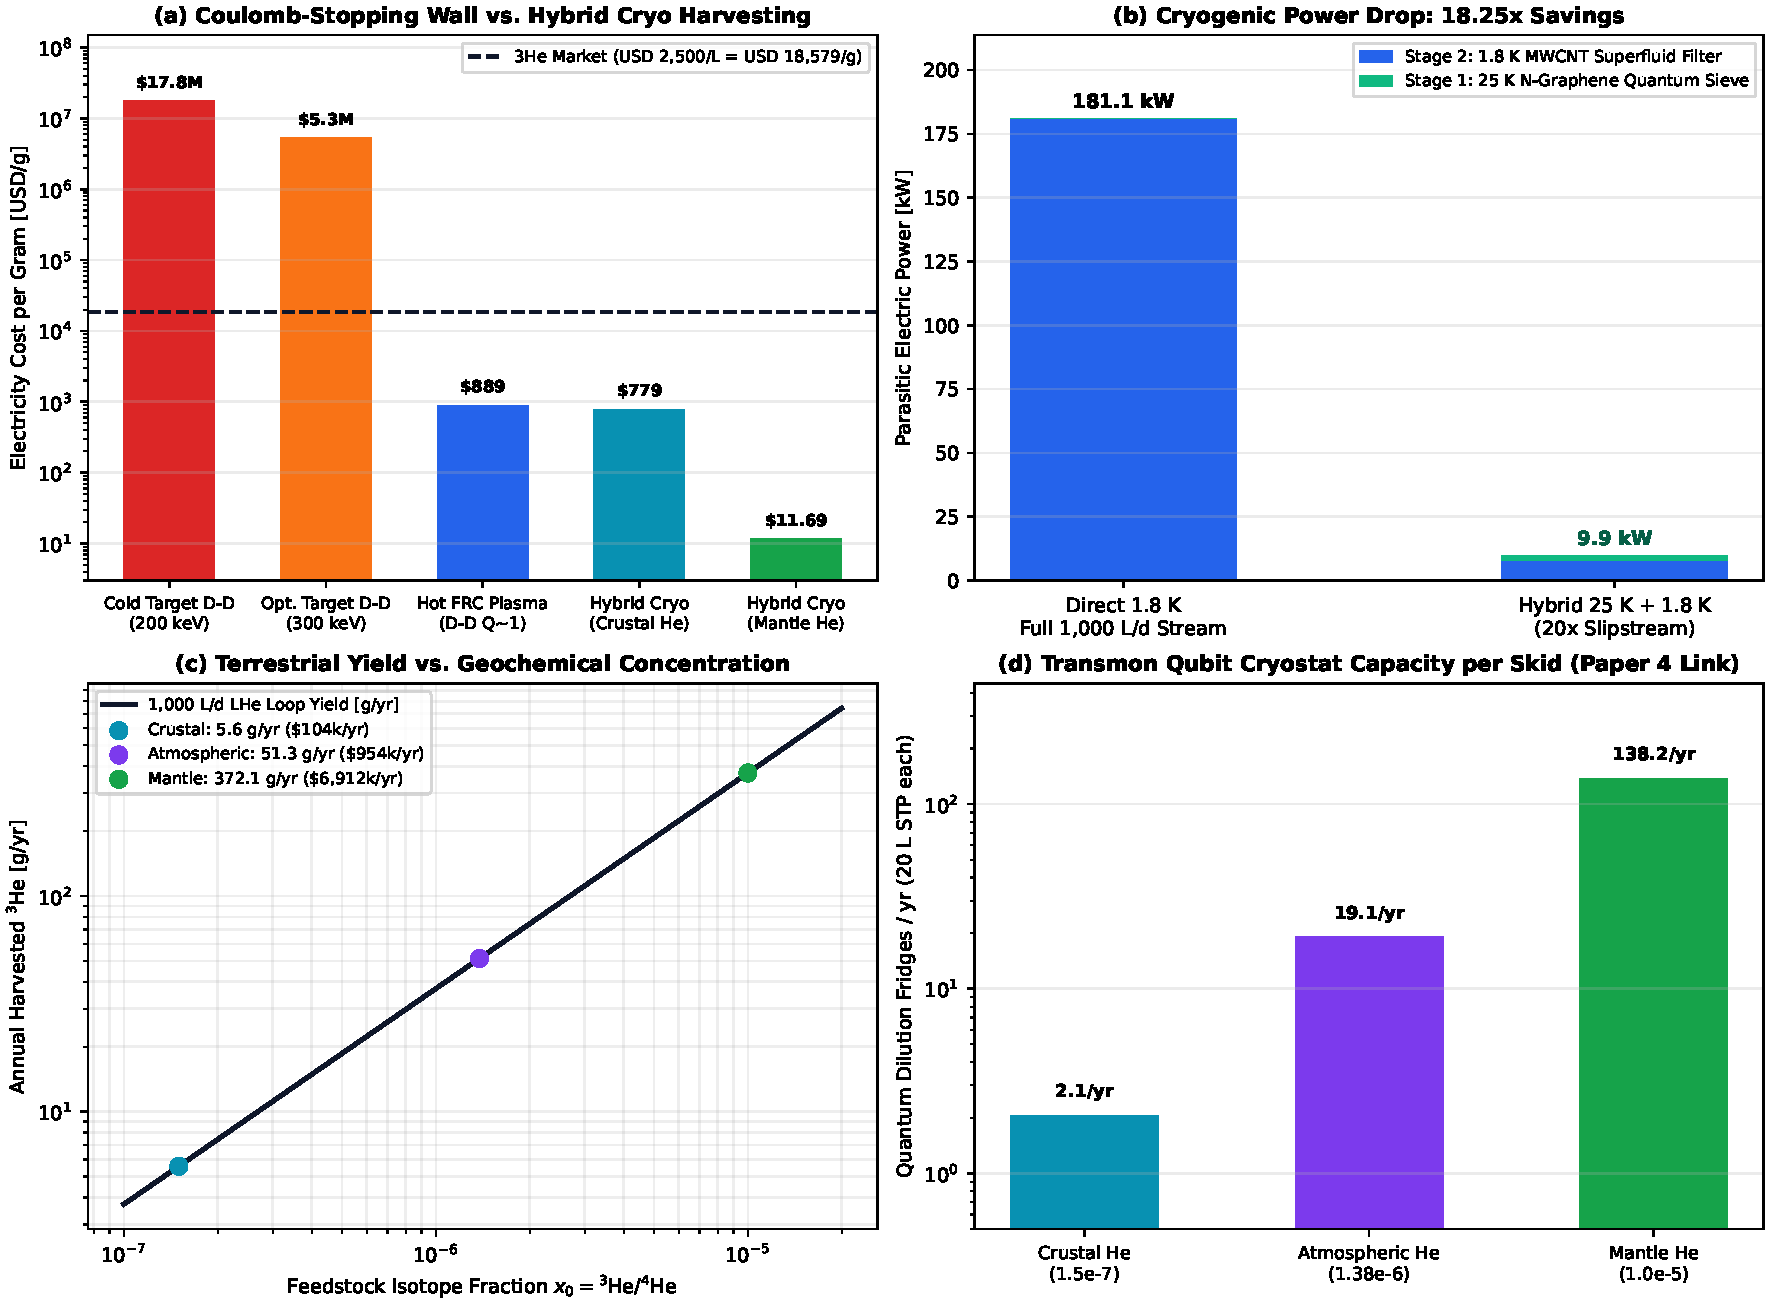
\includegraphics[width=\textwidth]{../figures/fig1_he3_terrestrial_exergy_audit.pdf}
\caption{First-principles exergy and supply audit of terrestrial $^3\mathrm{He}$ pathways: (a) electricity cost per gram across nuclear synthesis vs.\ hybrid cryogenic harvesting; (b) parasitic load drop ($18.25\times$) via $25\text{ K}$ graphene pre-concentration ahead of $1.8\text{ K}$ MWCNT superfluid filtration; (c) annual mass yield across geochemical concentrations; (d) quantum-computing dilution refrigerators supplied annually per $1{,}000\text{ L/day}$ skid.}
\label{fig:exergy}
\end{figure}

\section{Conclusion}
Non-lunar terrestrial $^3\mathrm{He}$ harvesting does not require infeasible cold-target accelerators or deep-ocean mantle mining. Coupling cryogenic nanoporous graphene pre-concentration ($T_1 \approx 25\text{ K}$) directly ahead of a sub-lambda MWCNT superfluid entropy filter ($T_2 = 1.8\text{ K}$) inside existing helium liquefaction streams cuts electrical power by $18.25\times$ to $9.92\text{ kW}$, yielding electricity-cost margins of $23.8\times$ on crustal helium and $1{,}589\times$ on mantle-enriched reservoirs while directly supplying quantum-computing cryogenics. Reproducible calculation modules, unit tests, and plotting code are open-source at \url{https://github.com/bruno-olivaes/he3-cryo-extractor}.

\bibliographystyle{unsrt}
\bibliography{refs}

\end{document}

